% Notas content

\begin{enumerate}
  \item Como é possı́vel determinar a massa efetiva dos semicondutores com o experimento de ressonância ciclotron? Discuta partindo da equação do movimento de Drude o que é a ressonância ciclotron, e a geometria/consequência experimental.\\

    Nós temos que a força de Loretenz é dada por:

    \begin{equation}
         \mathbf{F} = q(\mathbf{E} + v \times \mathbf{B}) 
    \end{equation}

    Considerando que o campo elétrico, $E$ seja igual a $0$, e usando a definição de força chegamos na expressão (estou negligenciando o termo de amortecimento que aparece na equação de drude, pois ele não irá alterar a frequência final, apenas o pico):

    \begin{equation}
        m^*\dv{v}{t} = q(v \times \mathbf{B}) 
    \end{equation}

    Supondo que temos um campo magnético uniforme na direção $\hat{z}$, ou seja: $\mathbf{B} = B\hat{z}$, podemos dizer então que $v \times B$ é dado por:

    $$(v_x, v_y, 0) \times (0, 0, B) = (v_yB, -v_xB, 0)$$
    Indicando que temos uma rotação no plano xy. Podemos separar as equações diferenciais de acordo com suas componentes, ficamos então com:
  \begin{center}
    $\begin{cases}
      m^*\dv{v_x}{dt} = q(v_yB)\\\\
      m^*\dv{v_y}{dt} = -q(v_xB)
    \end{cases}$
  \end{center}
  
  Podemos derivar a primeira equação diferencial mais uma vez, obtendo então:

  $$m^*\dv[2]{v_x}{t} = qB\dv{v_y}{t}$$
  Porém, sabemos que $\dv{v_y}{t} = -\frac{qB}{m^*}v_x$. Substituindo obtemos no final que:

  \begin{equation}
     \dv[2]{v_x}{t} = -\left(\frac{qB}{m^*}\right)^2v_x 
  \end{equation}

  A forma dessa equação diferencial é a mesma do oscilador harmônico que já resolvemos em aula, sendo assim, podemos definir uma frequência (que parece ser uma convenção nos livros) \textit{ciclotron}:

  \begin{equation}
      \omega^2 = \left(\frac{qB}{m^*}\right)^2 \Implies \omega = \frac{|q|B}{m^*} 
  \end{equation}
  
  No experimento de ressonância ciclotron, a intenção é aplicar um campo eletromagnético com uma frequência $\omega$ até que ela chegue na frequência ciclotron, pois ao terem a mesma frequência, elas entram em ressonância e absorção de energia do elétron é máxima. Nós não sabemos a frequência ciclotron, nem a massa efetiva, porém sabemos que se variarmos a frequência do campo eletromagnético que estamos emitindo, em um dado momento teremos um pico no gráfico $E \times \omega$, e é justamente esse pico que corresponde à frequência ciclotron. Dessa forma, sabendo a frequência, a carga do elétron e o campo magnético, podemos calcular a massa efetiva dos semicondutores.

\item Como é possı́vel determinar a concentração de portadores dos semicondutores usando medidas Hall? Discuta partindo da equação do movimento de Drude a consequência experimental da geometria Hall.


\begin{figure}[htbp]
  \centering
  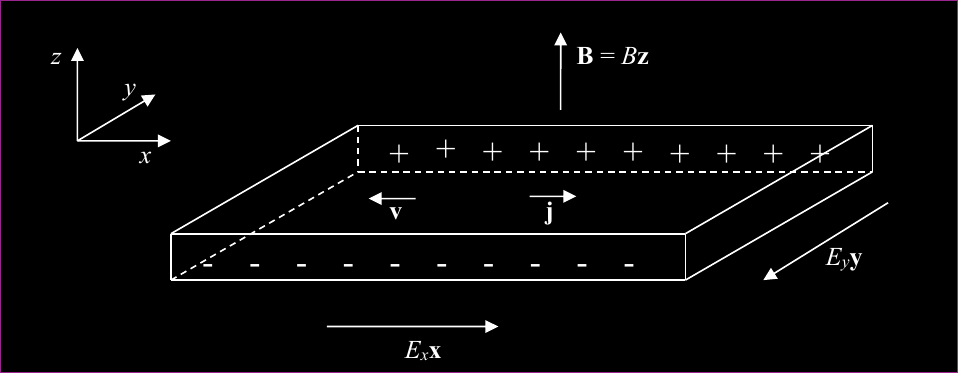
\includegraphics[width=\linewidth]{images/Hall experiment.png}
\end{figure}
  
A geometria do experimento Hall parte do pressuposto que temos dois campos sendo aplicados em nossa amostra, um campo elétrico sendo aplicado na direção +x, $E_x\hat{x}$ e um campo magnético sendo aplicado perpendiculamente, direção z, $\mathbf{B} = Bz$. O campo elétrico $E_x\hat{x}$ faz com que tenhamos uma corrente elétrica nesse sentido, $j$. Como temos um campo magnético sendo aplicado da direção z, ocorre uma defleção dos elétrons por conta da força de Lorentz. Sendo assim, cargas negativas começam a acumular de um lado da amostra. Essa diferença de cargas na parede faz com que surja um campo elétrico na direção $-E_y\hat{y}$, sendo assim, surje uma corrente elétrica, que seria a corrente de Hall.

Analisando esse experimento no regime estacionário, ou seja, quando $\dv{v_y}{t} = 0$, temos então que na direção y:

\begin{equation}
  0 = q(E_y + v_xB) \Implies E_y = -v_xB
\end{equation}

Onde o $E_y$ é justamente o nosso campo Hall. Sabemos que a densidade da corrente é $j = nqv_x$. Substituindo $v_x$ no campo de Hall, obtemos:

\begin{equation}
    E_y = -\frac{j_x}{nq}B 
\end{equation}

E o coeficiente Hall é definido como: 

\begin{equation}
    R_H = \frac{E_y}{j_xB} = - \frac{1}{nq} 
\end{equation}

Em um experimento Hall, conseguimos medir $E_y$ e nós já conhecemos a $j_x$ e $B$, afinal, eles são aplicados de maneira controlada. Sendo assim, podemos calcular o coeficiente Hall e usar a expressão que relaciona ele com a densidade dos portadores de carga:
\begin{equation}
R_H = -\frac{1}{nq} \Implies n = -\frac{1}{R_Hq}
\end{equation}

\item Interprete e explique a dependência da temperatura na densidade de portadores de carga para o Ge dopado tipo-n com diferentes contrações de dopantes $N_d$, figura abaixo.

  \begin{center}
\begin{figure}[htbp]
  \centering
  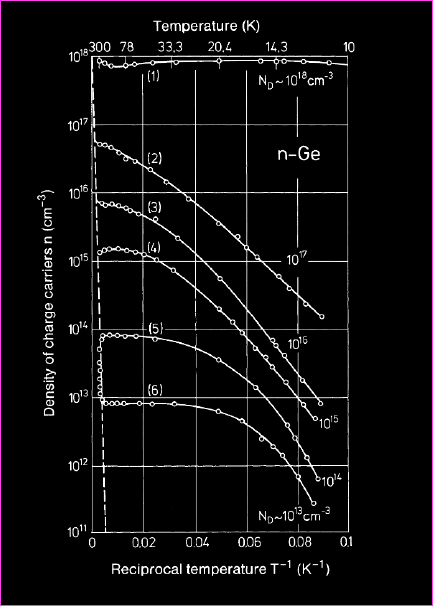
\includegraphics[scale=0.5]{images/Ge dopado.png}
\end{figure}
\end{center}
A primeira coisa que eu notei ao observar a imagem, é que no caso do nosso semicondutor puro, intrínseco, a densidade de portadores delétrons só começa a ser relevante a partir de altas temperatura. Supondo que a função que descreve a densidade dos portadores de elétrons seja contínua, e a "tendência" da função seja a mesma, é possível perceber que a densidade dos portadores de elétrons do semicondutor intrínseco para baixas temperaturas fica praticamente perto de zero, sendo negligenciável se comparado com sua versão dopada. Dessa forma, o nosso semicondutor à baixas temperaturas age basicamente como um isolante. Ao introduzirmos uma dopagem tipo-n no nosso Ge, temos mais elétrons disponíveis. Analisando o impacto da diferentes concentrações de dopantes e temperatura na densidade dos portadores de cargas, é possível notar-se algumas coisas. Primeiro, a é que parecem haver três "regimes" que determinam a densidade dos portadores de carga. Em baixas temperaturas, temos que $n << N_d$, e para baixas concentrações de $N_D$, o crescimento de $n$ com a temperatura parece ocorrer de maneira logarítima, até que chegamos à situação onde $n = N_D$. Nessa situação a variação de temperatura não afeta muito $n$, até que chegamos no regime de altas temperaturas e $n>N_D$. Nesse caso, podemos presumir que a temperatura foi o suficiente para ionizar os átomos, fazendo com que mais elétrons vão para a banda de condução, deixando buracos na banda de valência. É interessante notar que o aumento de concentração de dopantes faz com que o comportamento da função no gráfico $n \times K$ seja cada vez mais linear. Porém, quando chegamos em uma concentração tão alta de dopante, $N_D = 10^{18}$, praticamente a densidade de portadores de cargas é uma constante. Eu pressuponho que isso ocorre pelo fato da quantitade de elementos dopantes serem extremamente maiores do que a quantidade de átomos de Germânio.
  
\item {}
\end{enumerate}
